\documentclass{article}
\usepackage[utf8]{inputenc}
\usepackage{graphicx}
\usepackage{amsmath, amssymb, amsfonts}
\usepackage{geometry}
\usepackage{float}
\usepackage{hyperref}
\usepackage{enumitem}
\usepackage{caption}
\usepackage{subcaption}
\usepackage{color}
\usepackage{soul}
\usepackage{listings}
\usepackage{xcolor}
\usepackage{booktabs}
\usepackage{wasysym}

\geometry{a4paper, margin=1in}

\title{Methods in Computational Neuroscience:\\Firing rate models and dynamical systems}
\author{Sepehr SAEEDPOUR}
\date{\today}

\begin{document}

\maketitle

\section*{Introduction}
% Provide context about the assignment topic
In 1943, \emph{Warren McCulloch} and \emph{Walter Pitts} showed that a neuron can be treated like an “on–off’’ switch that fires only when its inputs cross a threshold, laying the first mathematical bricks for digital‐style brain models.
\emph{Donald Hebb} pushed the idea further in 1949 when he argued that connections between two switches grow stronger whenever they are active at the same time—a simple rule that hints at how learning might work.
In the early 1970s, \emph{Hugh Wilson} and \emph{Jack Cowan} replaced those binary switches with smooth firing-rate equations and used phase–plane diagrams and bifurcations to explain real cortical rhythms and steady states.

\emph{John Hopfield} showed in 1982 that a network with symmetric connections naturally settles into a handful of stable activity patterns that act as content‐addressable memories.  
His calculation revealed a sweet spot: with Hebbian wiring, an $N$-cell Hopfield network can reliably store roughly $0.138\,N$ random binary patterns.  
The trick behind these memories is positive feedback: when neurons excite themselves or each other strongly enough through an S-shaped, sigmoidal response curve, the circuit can flip between "off" and "on" states and stay there after the original input disappears—an effect called \emph{bistability}. 

This report shows how these ideas develop, starting from a single neuron and expanding to a full Hopfield network.
First, we will see how a \emph{single self-connected neuron} can behave like a tiny memory switch whose state survives noise.  
Next, we will analyse a \emph{pair of mutually exciting neurons} and watch how their interaction carves the plane into two attractor basins separated by a saddle.  
Finally, the ideas scale up to a \emph{64-unit Hopfield network} where we measure storage limits, draw energy landscapes, and test how well the network corrects errors.  
By the end, we will have traced one continuous thread—from early logic gates to attractor networks showing how simple equations can capture the brain’s ability to store, retrieve and protect information over time.


\section{Neuron with self-connection}

\subsection{Plot the activation function}
% Description of the first task/analysis

The activation function $f(s) = 60(1 + \tanh(s))$ maps the total input to the neuron's firing rate. 
This sigmoidal function has several key properties: output range of $[0, 120]$ spikes per second, centered at $f(0) = 60$ spikes per second, and asymptotic behavior approaching 0 for very negative inputs and 120 for very positive inputs. 



\begin{figure}[H]
    \centering
    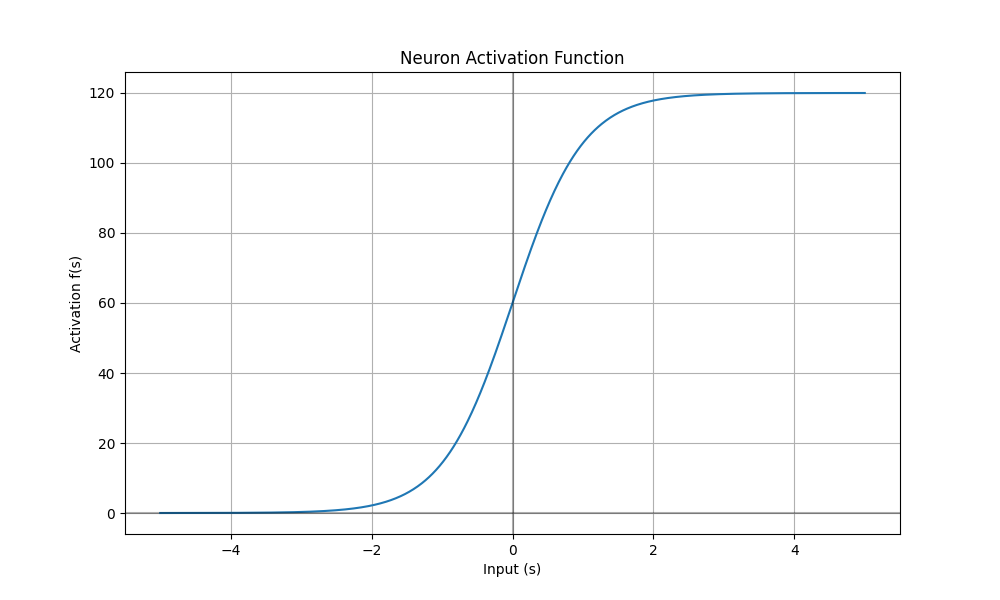
\includegraphics[width=0.5\textwidth]{activation_function.png}
    \caption{Plot of the activation function $f(s) = 60(1 + \tanh(s))$ over the input range $[-5, 5]$. The function shows the characteristic S-shape of a sigmoid, with output values ranging from 0 to 120 spikes per second.}
    \label{fig:activation}
\end{figure}

\subsection{Study the dynamics}

When simulating the system with three initial conditions $r(0) = 59$, $r(0) = 60$, and $r(0) = 61$, I observe interesting dynamical behavior:

\begin{itemize}
    \item For $r(0) = 59$: The firing rate decreases and settles at the lower stable fixed point.
    \item For $r(0) = 60$: The firing rate remains constant, indicating this is an unstable fixed point.
    \item For $r(0) = 61$: The firing rate increases and settles at the higher stable fixed point.
\end{itemize}

This behavior indicates the system has three fixed points, with the middle one ($r \approx 60$) acting as a threshold. Initial conditions below this threshold lead to a low firing rate state, while initial conditions above it lead to a high firing rate state. This is characteristic of a bistable system.

\begin{figure}[H]
    \centering
    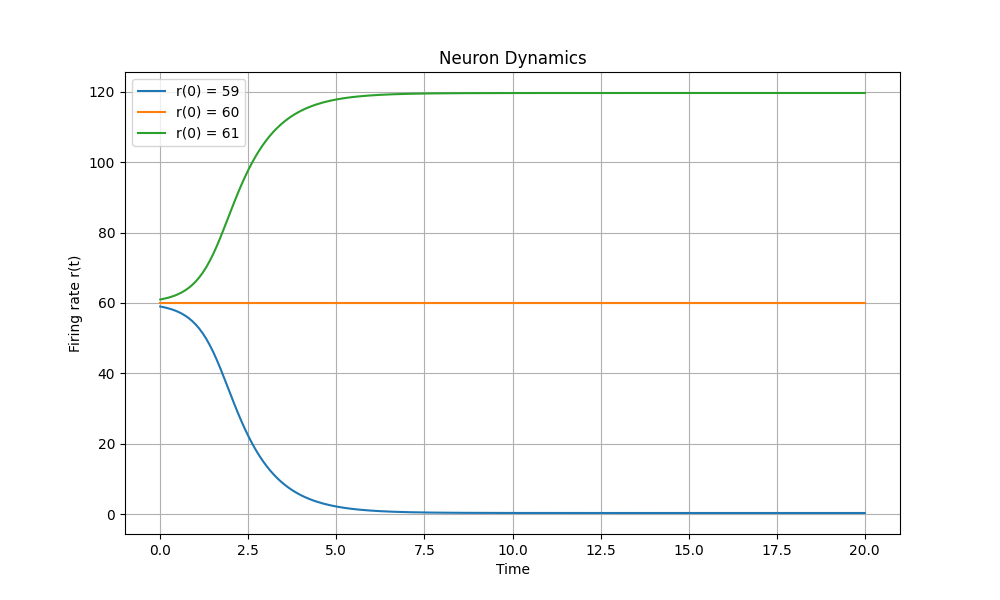
\includegraphics[width=0.5\textwidth]{deterministic_dynamics.png}
    \caption{Time evolution of the neuron firing rate $r(t)$ with three different initial conditions: $r(0) = 59$, $r(0) = 60$, and $r(0) = 61$. The trajectories demonstrate the bistable nature of the system, with two stable fixed points separated by an unstable threshold at $r \approx 60$.}
    \label{fig:deterministic}
\end{figure}

\subsection{Add noise}

Adding noise to the system reveals additional insights:

\begin{equation}
\frac{dr(t)}{dt} = -r(t) + f(wr(t) + I) + \sigma\eta(t)
\end{equation}

Where $\eta(t)$ is Gaussian white noise and $\sigma$ is the noise magnitude.

\begin{itemize}
    \item \textbf{(a)~Low noise} ($\sigma = 0.1$): The system mostly maintains its bistable behavior, exhibiting only small stochastic excursions around the two attracting fixed points.  A trajectory that starts near $r_0 \!\approx\! 60\,$Hz drifts away because this intermediate firing rate is an \emph{unstable} fixed point, so the rate does \emph{not} remain constant there. 
    \item \textbf{(b)~Medium noise} ($\sigma = 5.0$): Larger fluctuations occasionally push trajectories across the separatrix, so the neuron sometimes switches between zero and high-firing states.
    \item \textbf{(c)~High noise} ($\sigma = 20.0$): Noise dominates the dynamics; trajectories hop back and forth between the two attractors so frequently that the system effectively loses any memory of its initial condition.
\end{itemize}

This demonstrates how noise can induce transitions between stable states in a bistable system, with the frequency of transitions increasing with noise magnitude.

\begin{figure}[H]
    \centering
    \begin{subfigure}[b]{0.48\textwidth}
        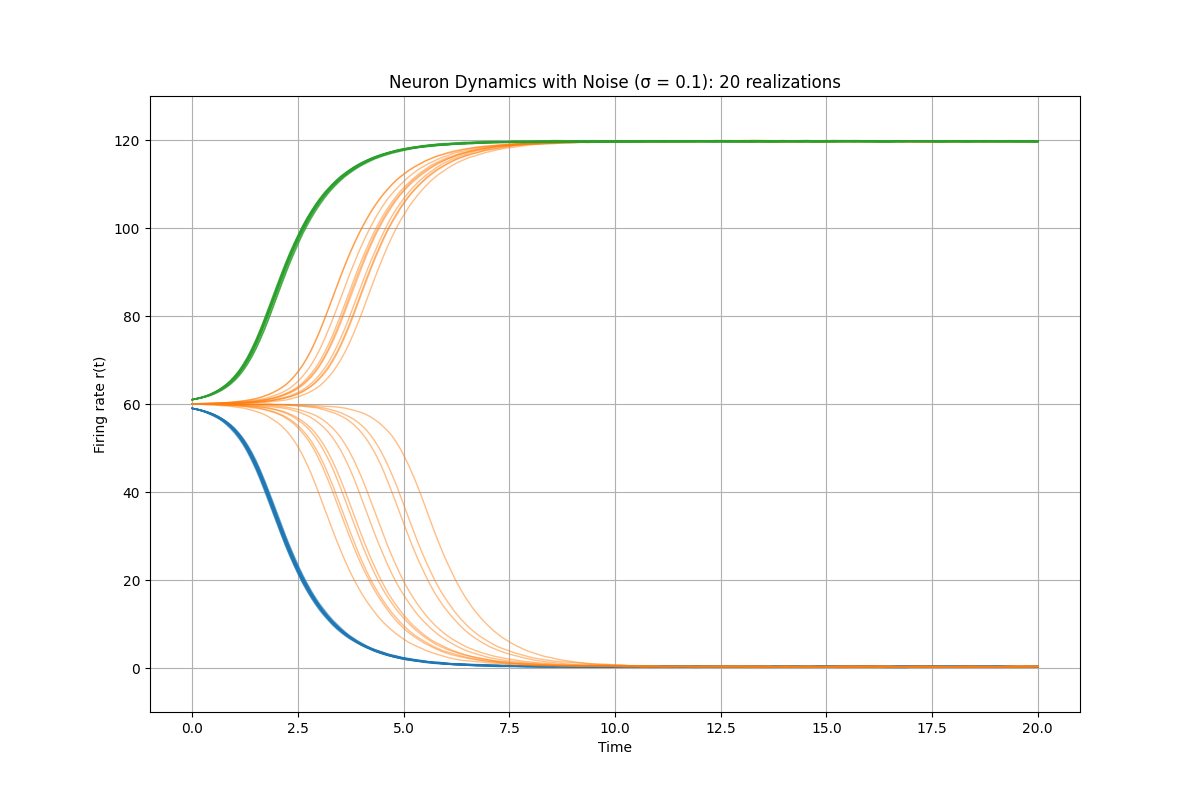
\includegraphics[width=\textwidth]{noise_strength_0.1.png}
        \caption{Low noise ($\sigma = 0.1$)}
        \label{fig:noise_low}
    \end{subfigure}
    \hfill
    \begin{subfigure}[b]{0.48\textwidth}
        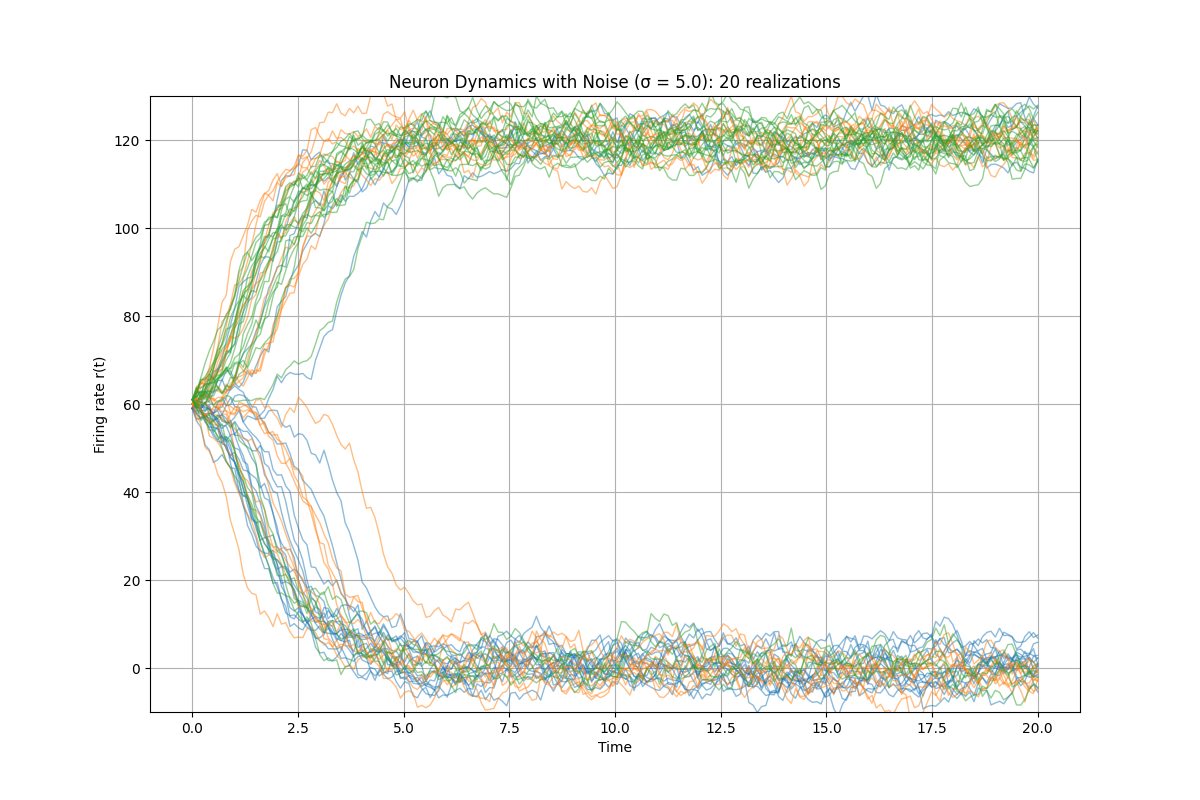
\includegraphics[width=\textwidth]{noise_strength_5.0.png}
        \caption{Medium noise ($\sigma = 1.0$)}
        \label{fig:noise_medium}
    \end{subfigure}
    
    \vspace{0.3cm}
    \begin{subfigure}[b]{0.48\textwidth}
        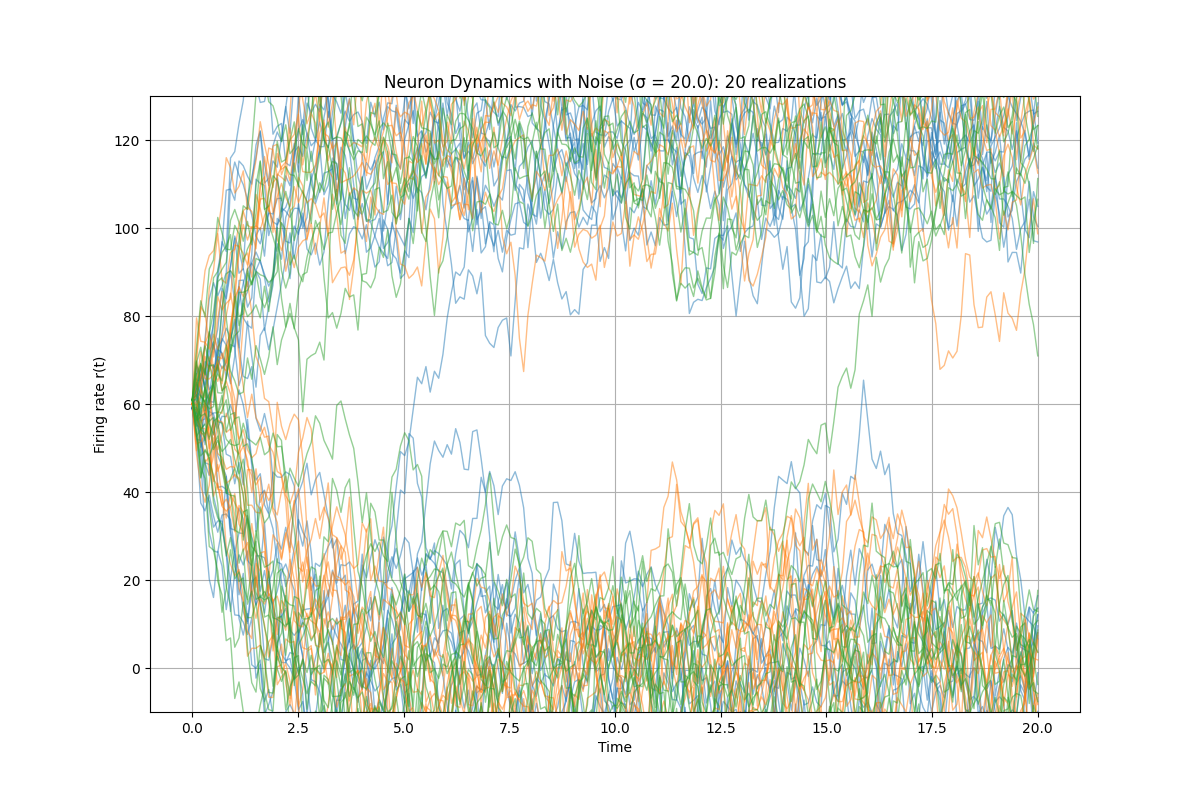
\includegraphics[width=\textwidth]{noise_strength_20.0.png}
        \caption{High noise ($\sigma = 20.0$)}
        \label{fig:noise_high}
    \end{subfigure}
    \caption{Effect of different noise levels on the neuron dynamics. As noise magnitude increases, transitions between stable states become more frequent, demonstrating how noise can induce state switching in a bistable system.}
    \label{fig:noise_effects}
\end{figure}


\subsection{Study the flux}


The flux analysis examines the derivative $\frac{dr}{dt}$ as a function of the firing rate $r$. The plot of this flux function reveals:

\begin{itemize}
    \item Three zero-crossings (fixed points) where $\frac{dr}{dt} = 0$:
    \begin{enumerate}
        \item Lower fixed point: Stable (negative slope at crossing)
        \item Middle fixed point: Unstable (positive slope at crossing)
        \item Upper fixed point: Stable (negative slope at crossing)
    \end{enumerate}
\end{itemize}

The stability of these fixed points can be determined by the slope of the flux function at each crossing:
\begin{itemize}
    \item Negative slope: Stable fixed point (perturbing the system slightly causes it to return to the fixed point)
    \item Positive slope: Unstable fixed point (perturbing the system slightly causes it to move away from the fixed point)
\end{itemize}

These findings confirm our observations from the time series simulations, providing a deeper understanding of the bistable nature of the system.

\begin{figure}[H]
    \centering
    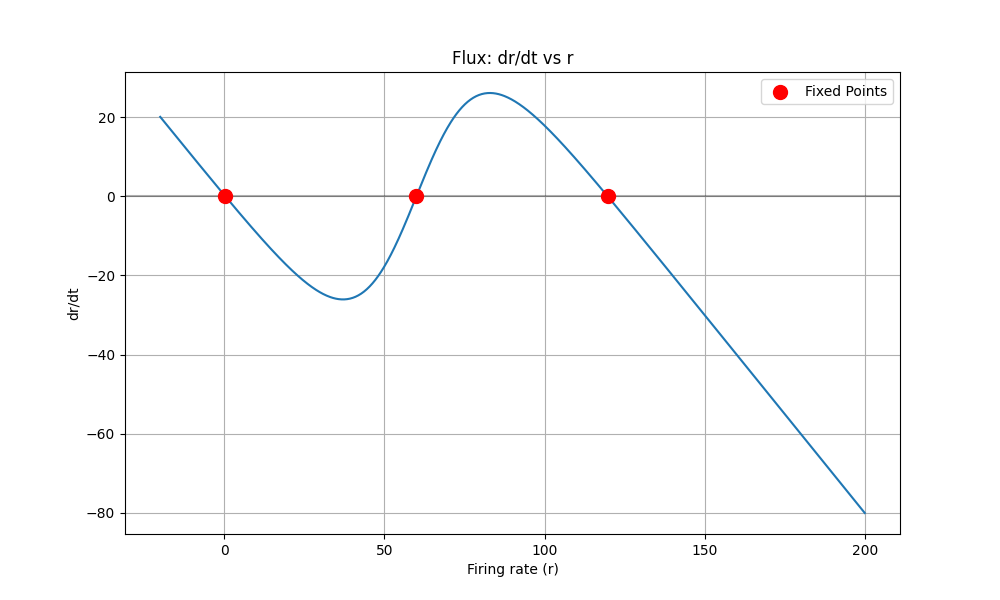
\includegraphics[width=0.5\textwidth]{flux_analysis.png}
    \caption{Flux analysis showing $\frac{dr}{dt}$ as a function of firing rate $r$. The zero-crossings represent fixed points of the system. The middle fixed point has a positive slope (unstable), while the other two have negative slopes (stable), confirming the bistable nature of the system.}
    \label{fig:flux}
\end{figure}


\subsection{Bifurcation diagram}

The bifurcation diagram explores how the number and nature of fixed points change as system parameters (synaptic strength $w$ and external input $I$) vary. The analysis reveals:

\begin{itemize}
    \item For low values of $w$ (weak self-connection): The system has a single stable fixed point.
    \item For higher values of $w$: The system exhibits bistability with three fixed points (two stable, one unstable).
\end{itemize}



\begin{figure}[H]
    \centering
    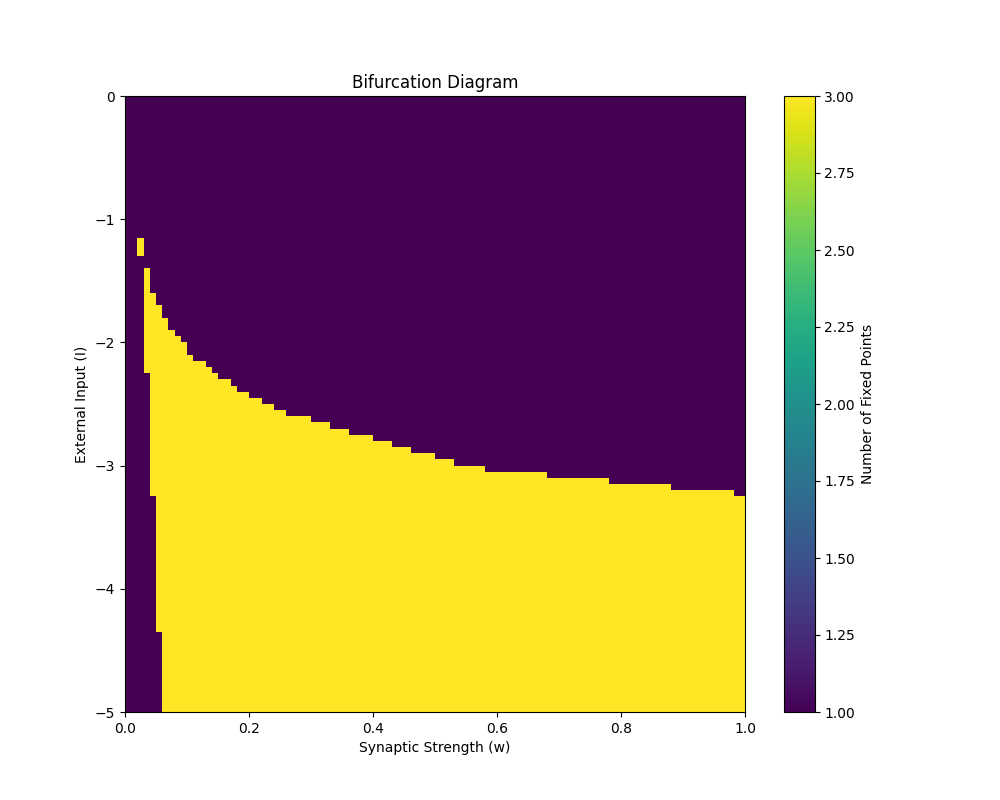
\includegraphics[width=0.5\textwidth]{bifurcation_diagram.png}
    \caption{Bifurcation diagram showing how the number of fixed points changes with synaptic strength ($w$) and external input ($I$). Different colors represent different numbers of fixed points. The boundaries between regions represent bifurcation points where the qualitative behavior of the system changes.}
    \label{fig:bifurcation}
\end{figure}




\section{2D network: mutual excitation}

\subsection{Plot the dynamics}

The time evolution of the firing rates $x(t)$ and $y(t)$ was simulated for different initial conditions. The differential equations were integrated numerically using the Euler method with a time step of $dt = 0.1$.

Figure 6 shows the evolution of the firing rates over time for four different initial conditions.


\begin{figure}[H]
    \centering
    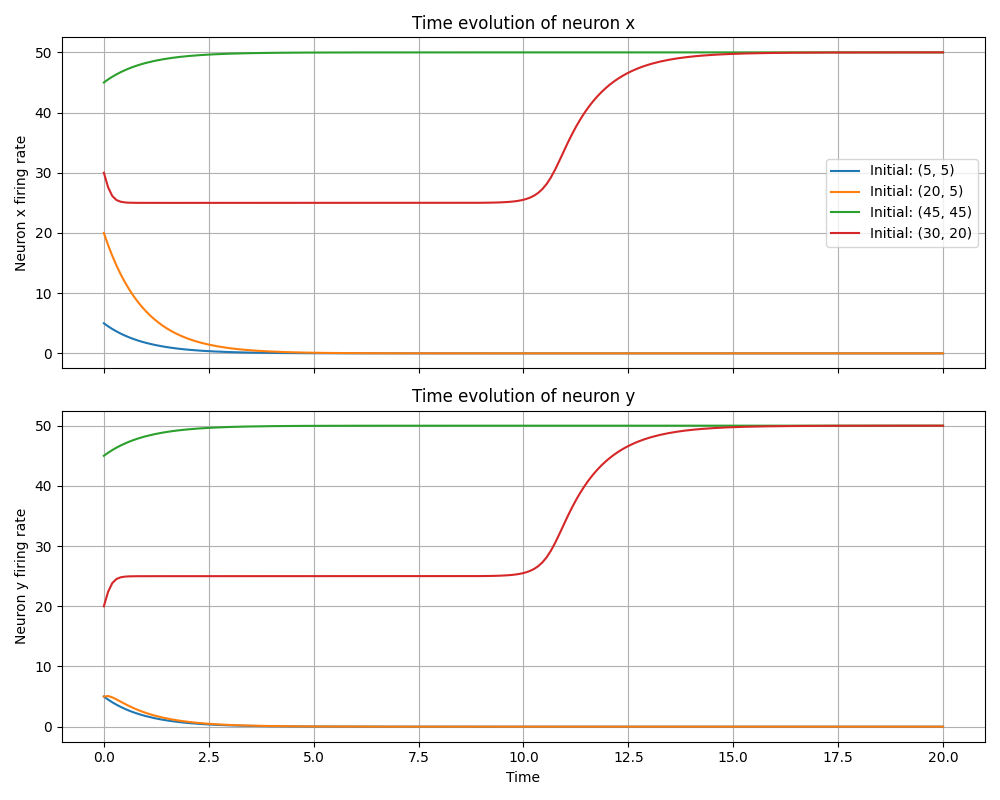
\includegraphics[width=0.5\textwidth]{dynamics2_plot.png}
    \caption{Time evolution of the firing rates $x(t)$ and $y(t)$ for different initial conditions. The top panel shows the firing rate of neuron $x$, and the bottom panel shows the firing rate of neuron $y$.}
    \label{fig:dynamics}
\end{figure}

From the time evolution plots, we can observe that:
\begin{itemize}
    \item Initial conditions starting near $[5, 5]$ converge to zero firing rates (both neurons shut down).
    \item Initial conditions starting near $[45, 45]$ converge to a high firing rate fixed point.
    \item The middle-low and mixed initial states show interesting transient dynamics before eventually converging to either zero firing rate or a high firing rate fixed point.
\end{itemize}

This suggests that the system exhibits bistability, with two stable fixed points (attractors) and a saddle point that separates their basins of attraction.

\subsection{State space}


The trajectories in state space (plotting $x$ versus $y$) provide a more comprehensive view of the dynamics. Figure 7 shows these trajectories for seven different initial conditions.

\begin{figure}[H]
    \centering
    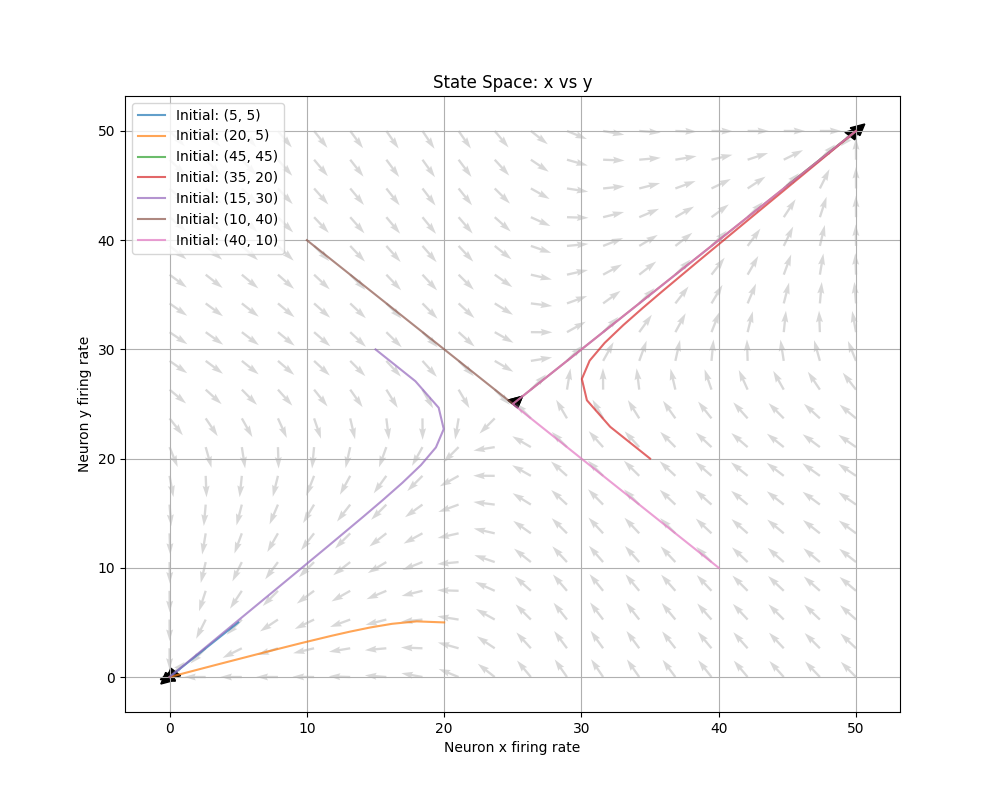
\includegraphics[width=0.65\textwidth]{state_space2.png}
    \caption{State space trajectories for different initial conditions. Arrows indicate the direction of movement along each trajectory. They show that trajectories starting on one side of the saddle’s stable manifold flow to the low-rate rest state, while those on the other side are driven to the high-rate self-excited state, revealing bistability.}
    \label{fig:state_space}
\end{figure}

\subsection{Nullclines}

Nullclines are curves in the state space where the derivative of one variable is zero. For this system:
\begin{itemize}
    \item $x$-nullcline: $\frac{dx}{dt} = 0 \implies x = f(w_2 y + I) = f(0.4y - 10)$
    \item $y$-nullcline: $\frac{dy}{dt} = 0 \implies y = f(w_1 x + I) = f(0.4x - 10)$
\end{itemize}

Figure 8 shows the nullclines plotted in the state space.

\begin{figure}[H]
    \centering
    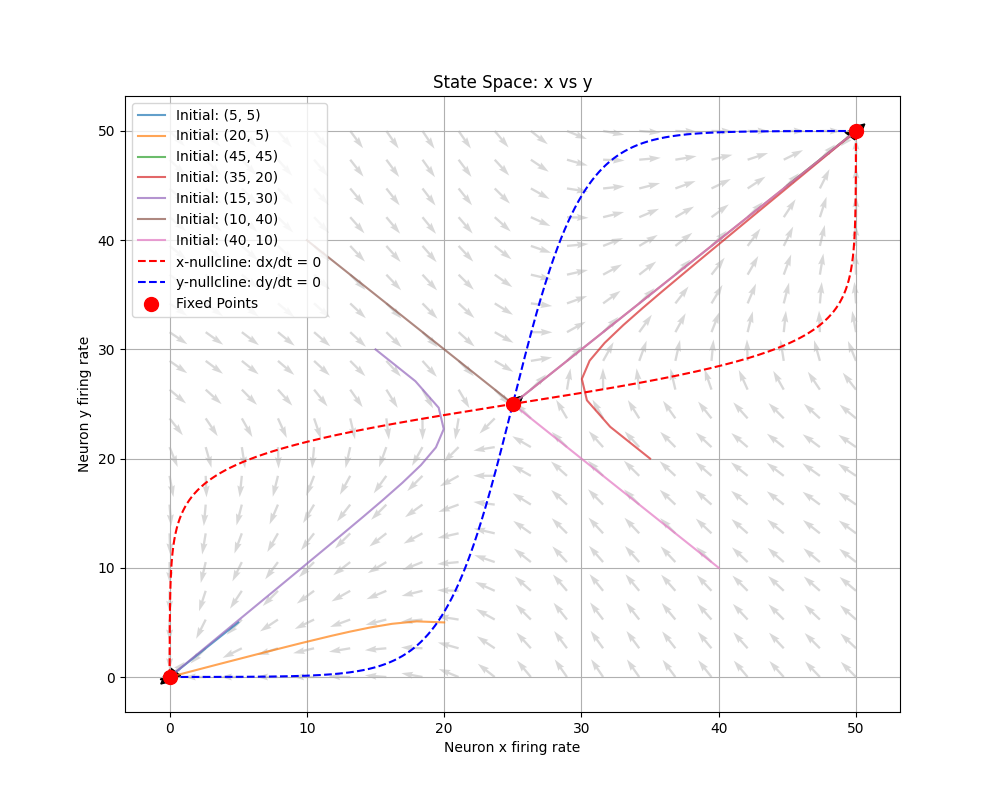
\includegraphics[width=0.65\textwidth]{state_space2_fixed_points.png}
    \caption{Nullclines of the system. The red dashed line represents the $x$-nullcline ($dx/dt = 0$), the blue dashed line represents the $y$-nullcline ($dy/dt = 0$), and red dots represent fixed points. }
    \label{fig:nullclines}
\end{figure}

Along the red \(x\)-nullcline (\(\dot{x}=0\)) the horizontal flow changes sign—
arrows point left (\(\dot{x}<0\)) to its left and right (\(\dot{x}>0\)) to its right—
while along the blue \(y\)-nullcline (\(\dot{y}=0\)) the vertical flow is upward
(\(\dot{y}>0\)) below and downward (\(\dot{y}<0\)) above.
Because the sigmoid is S-shaped, the nullclines bend sharply around the threshold
\(0.4(\text{x or y})-10=25\).
\subsection{Fixed points}
The fixed points of the system are located at the intersections of the nullclines (Figure 8). Solving the system numerically:
\begin{equation}
\begin{cases}
x = f(0.4y - 10)\\
y = f(0.4x - 10)
\end{cases}
\end{equation}

We find three fixed points:
\begin{enumerate}
    \item Low firing rate fixed point: approximately at $[x, y] \approx [0, 0]$
    \item Middle firing rate fixed point: approximately at $[x, y] \approx [25, 25]$
    \item High firing rate fixed point: approximately at $[x, y] \approx [50, 50]$
\end{enumerate}

% \begin{figure}[H]
%     \centering
%     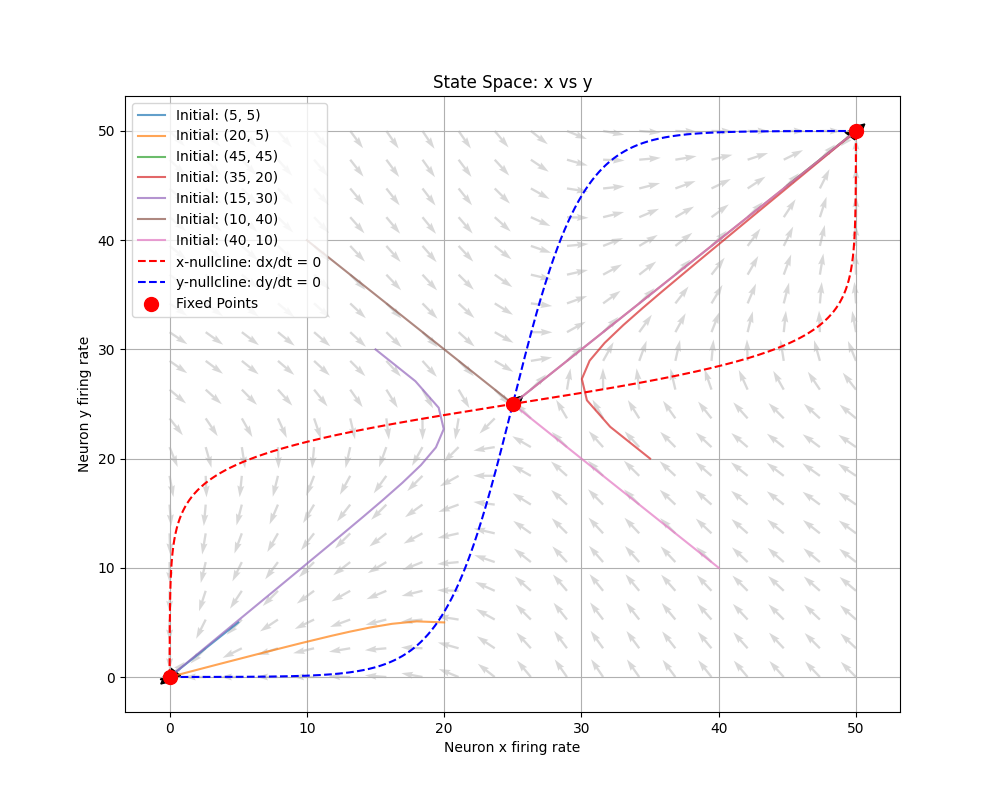
\includegraphics[width=0.5\textwidth]{state_space2_fixed_points.png}
%     \caption{State space with trajectories (solid lines), nullclines (dashed lines), and fixed points (red dots).}
%     \label{fig:state_space_nullclines_fp}
% \end{figure}

\begin{itemize}
    \item \textbf{Stable attractors.}  Trajectories drift toward the low-rate node near zero and toward the high-rate node close to saturation, demonstrating that both equilibria are stable.
    \item \textbf{Unstable saddle.} At moderate activity the trajectories reach a fixed point that is stable along one manifold (y = -x) and unstable along the orthogonal one (y = x). This exactly aligns with the signature of a saddle.
  \end{itemize}
  
  \noindent
  The state-space therefore contains two attracting fixed points—one at low (\(x=y\approx0\))
  and one at high (\(x=y\approx50\)) firing rates separated by an unstable saddle at
  \(x=y=25\).  State-space trajectories illustrate how every initial
  condition eventually settles into one of the two attractors, with the
  saddle acting as a boundary between them.

\subsection{Study the stability of the fixed points analitically}
To analyze the stability of the fixed points analytically, we compute the Jacobian matrix of the system:

\begin{equation}
J = 
\begin{bmatrix}
\frac{\partial}{\partial x}\left(-x + f(w_2 y + I)\right) & \frac{\partial}{\partial y}\left(-x + f(w_2 y + I)\right) \\
\frac{\partial}{\partial x}\left(-y + f(w_1 x + I)\right) & \frac{\partial}{\partial y}\left(-y + f(w_1 x + I)\right)
\end{bmatrix}
=
\begin{bmatrix}
-1 & w_2 f'(w_2 y + I) \\
w_1 f'(w_1 x + I) & -1
\end{bmatrix}
\end{equation}

where $f'(s) = \frac{df}{ds} = 50\sigma(s)(1 - \sigma(s))$, the derivative of our activation function.

For each fixed point $(x^*,y^*)$, we evaluate the Jacobian and determine its eigenvalues:
\[
\lambda_{1,2} = \frac{\text{tr}(J)}{2} \pm \sqrt{\frac{(\text{tr}(J))^2}{4} - \det(J)}
\]

The stability of each fixed point is determined by the eigenvalues:
\begin{itemize}
    \item If all eigenvalues have negative real parts, the fixed point is stable (attractor)
    \item If any eigenvalue has a positive real part, the fixed point is unstable
    \item If eigenvalues have opposite signs, the fixed point is a saddle point
\end{itemize}

Fixed point classification based on the determinant and trace:
\begin{itemize}
    \item $\det(J) < 0$: Saddle point (unstable)
    \item $\det(J) > 0, \text{tr}(J) < 0$: Stable node or spiral
    \item $\det(J) > 0, \text{tr}(J) > 0$: Unstable node or spiral
\end{itemize}

At the low fixed point $(x^*,y^*) \approx (0,0)$, the derivatives $f'$ are nearly zero because inputs are far below threshold, making $\det(J) \approx 1$ and $\text{tr}(J) \approx -2$, yielding eigenvalues $\lambda_{1,2} \approx -1$. This confirms it's a stable node.

At the middle fixed point $(x^*,y^*) \approx (25,25)$, the derivatives $f'$ are near maximum, and with $w_1=w_2=0.4$, we get $\det(J) = -24 < 0$, confirming it's a saddle point with one positive (4) and one negative (-6) eigenvalue.

At the high fixed point $(x^*,y^*) \approx (50,50)$, similar to the low fixed point, the derivatives are small as inputs are far above threshold, giving $\det(J) > 0$ and $\text{tr}(J) < 0$, confirming it's a stable node.

\begin{table}[H]
\centering
\begin{tabular}{@{}lccc@{}}
\toprule
\textbf{Fixed Point} & \textbf{Eigenvalues} & \textbf{Determinant} & \textbf{Classification} \\
\midrule
Low $(0,0)$ & Both negative & Positive & Stable node \\
Middle $(25,25)$ & One positive, one negative & Negative & Saddle point \\
High $(50,50)$ & Both negative & Positive & Stable node \\
\bottomrule
\end{tabular}
\caption{Stability analysis results for the three fixed points. The bistable behavior arises from having two stable nodes separated by a saddle point.}
\label{tab:stability}
\end{table}

This analytical stability analysis confirms our observations from the state space trajectories and explains the system's bistable behavior, with the saddle point forming the boundary between the basins of attraction of the two stable states.

\subsection{Bifurcation diagram}

The bifurcation diagram shows how the number and position of fixed points change as the external input current $I$ varies from $-20$ to $-10$.

\begin{figure}[H]
    \centering
    \begin{subfigure}{0.48\textwidth}
        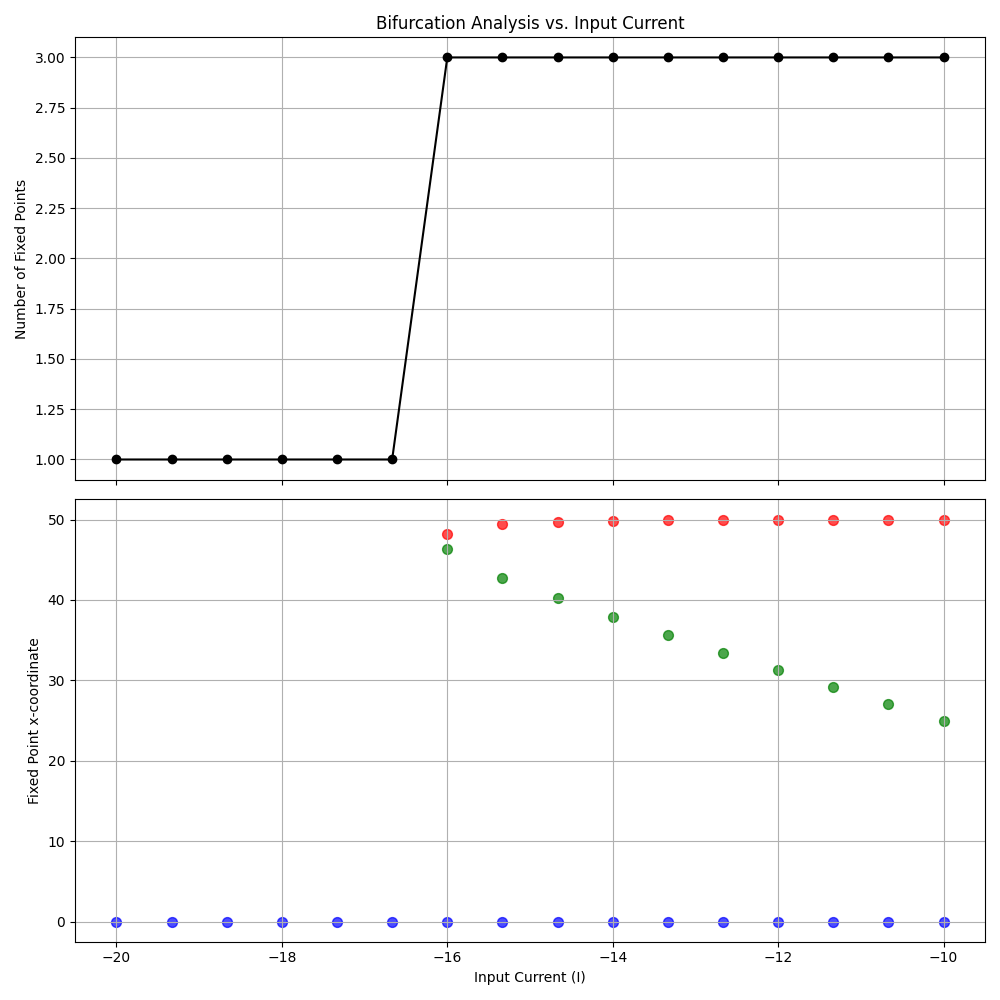
\includegraphics[width=\textwidth]{bifurcation_analysis_22.png}
        \caption{Bifurcation diagram showing the number of fixed points (top) and the $x$-coordinates of fixed points (bottom) as a function of external input $I$.}
        \label{fig:bifurcation_matrix}
    \end{subfigure}
    \hfill
    \begin{subfigure}{0.48\textwidth}
        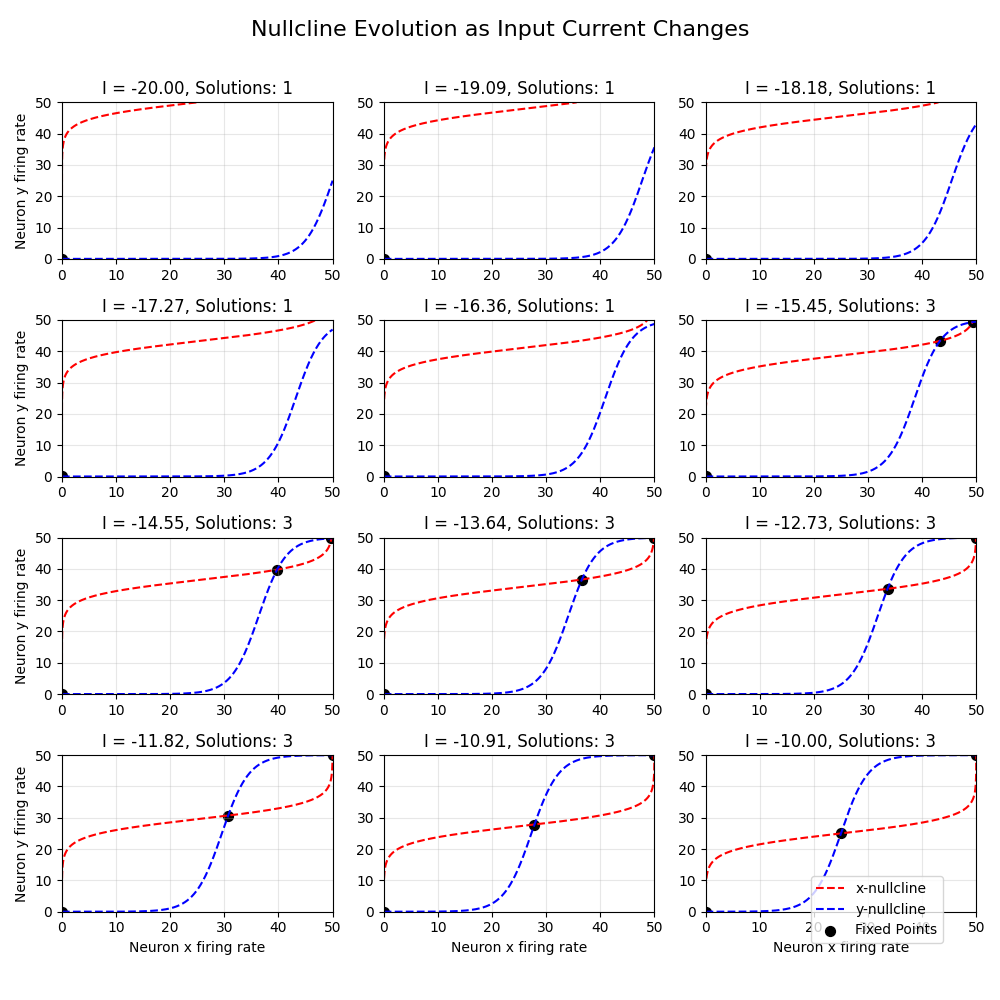
\includegraphics[width=\textwidth]{nullcline_evolution_2.png}
        \caption{Evolution of nullclines as $I$ changes. The intersections of nullclines are fixed points of the system, showing how they emerge with changing input.}
        \label{fig:nullcline_evolution}
    \end{subfigure}
    \caption{Analysis of system dynamics as a function of external input current $I$.}
    \label{fig:bifurcation_analysis_combined}
\end{figure}

\bigskip
From the bifurcation diagram, we observe how the fixed point structure changes with input current $I$. The bifurcation point occurs at approximately $I \approx -16$ where saddle-node bifurcation takes place.


From the bifurcation diagram, we can identify distinct regimes:
\begin{itemize}
    \item For very negative input ($I < -16$ approximately), there is only one stable fixed point with zero firing rate.
    \item For less negative input values ($-16 < I $ approximately), there are three fixed points: two stable (low (zero) and high firing rates) and one unstable (saddle point).

\end{itemize}

The system exhibits bistability in the intermediate range of input currents. 




\section{ND network: Hopfield neural network}


\subsection{Invent a pattern}

I begun by creating a specific pattern to store in our Hopfield network. For this experiment, I chose to create a simple 'X' pattern in an 8×8 grid. Each element in the pattern is either +1 or -1, represented visually as white or black pixels.

\begin{figure}[H]
\centering
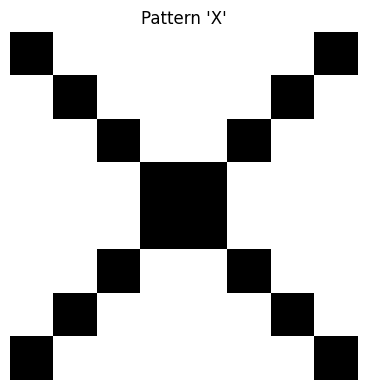
\includegraphics[width=0.3\textwidth]{Pattern 'X'.png}
\caption{Visual representation of the 'X' pattern stored in the network.}
\label{fig:pattern}
\end{figure}

The pattern is created as a 64-dimensional vector where each component takes the value +1 or -1 and is stored in the network's connectivity matrix using the outer product rule:

\begin{equation}
W_{ij} = \frac{1}{N}p_i p_j
\end{equation}

\subsection{Plot W and simulate the dynamics}
After storing the pattern, we can visualize the weight matrix $W$, which encodes the synaptic connections between neurons. The weight matrix is constructed using the outer product of the pattern with itself, divided by the number of neurons (64):

\begin{figure}[H]
\centering
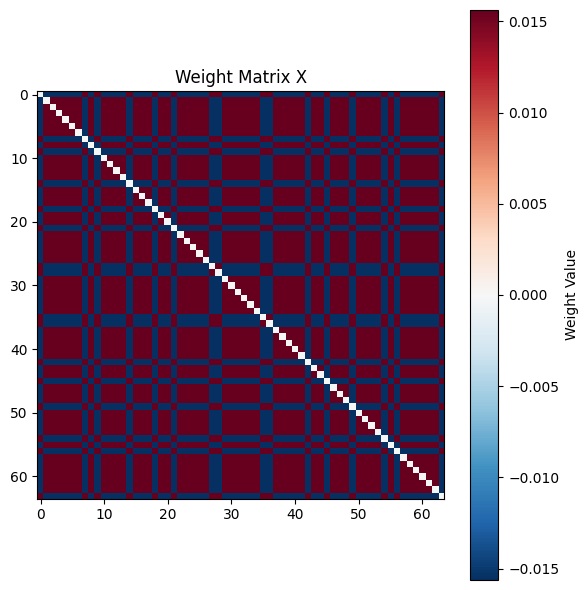
\includegraphics[width=0.3\textwidth]{Weight Matrix X.png}
\caption{Visualization of the weight matrix after storing the 'X' pattern. Red indicates positive weights, blue indicates negative weights.}
\label{fig:weight_matrix}
\end{figure}

The weight matrix shows the correlations between neurons based on the stored pattern. Strong positive connections (red) appear between neurons that have the same value in the pattern, while strong negative connections (blue) form between neurons with opposite values

To simulate the dynamics of the Hopfield network, we implement an Euler integration method with the following update rule:
\begin{equation}
x(t+\Delta t) = x(t) + \Delta t \cdot [-x(t) + f(Wx(t))] + \sigma\eta(t)\sqrt{\Delta t}
\end{equation}

where $\Delta t = 0.1$ is the time step, and $\sigma = 0.1$ is the noise amplitude.

Starting from random initial conditions, we examine how the network evolves over time:

\begin{figure}[H]
\centering
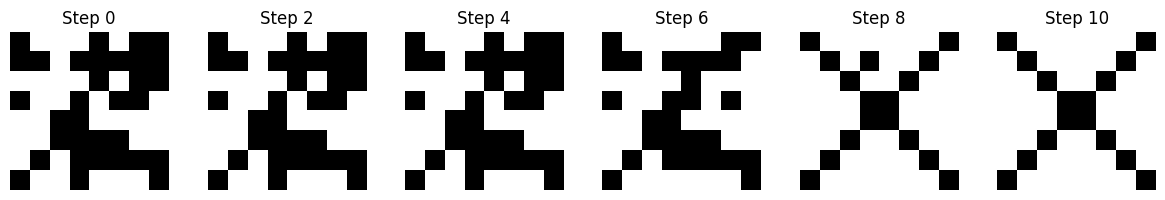
\includegraphics[width=0.9\textwidth]{Network Activity X.png}
\caption{Evolution of network activity from random initial conditions. The network converges to the stored 'X' pattern.}
\label{fig:network_dynamics}
\end{figure}

The figure illustrates the temporal evolution of the network state from random initial conditions. Over time, the network activity converges toward the stored pattern, demonstrating the attractor dynamics of Hopfield networks.




\subsection{Fixed points}


Running multiple simulations with different random initial conditions reveals consistent convergence behavior:

\begin{figure}[H]
\centering
\begin{subfigure}{0.2\textwidth}
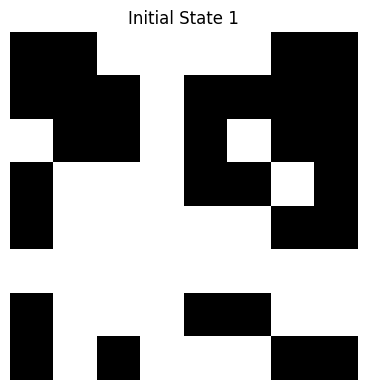
\includegraphics[width=\textwidth]{Initial State 1.png}
\caption{Initial State 1}
\end{subfigure}
\begin{subfigure}{0.2\textwidth}
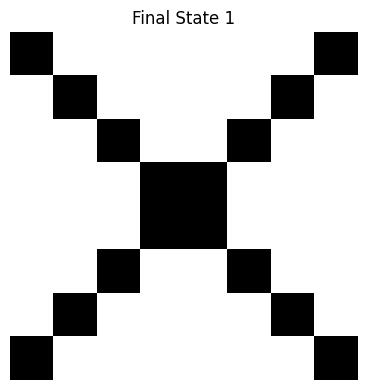
\includegraphics[width=\textwidth]{Final State 1.png}
\caption{Final State 1}
\end{subfigure}

\begin{subfigure}{0.2\textwidth}
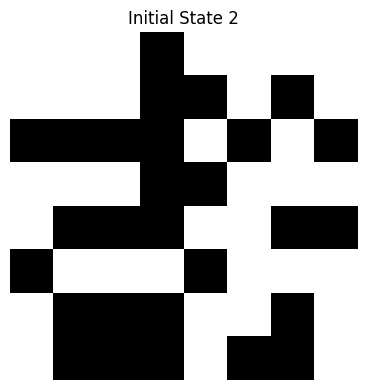
\includegraphics[width=\textwidth]{Initial State 2.png}
\caption{Initial State 2}
\end{subfigure}
\begin{subfigure}{0.2\textwidth}
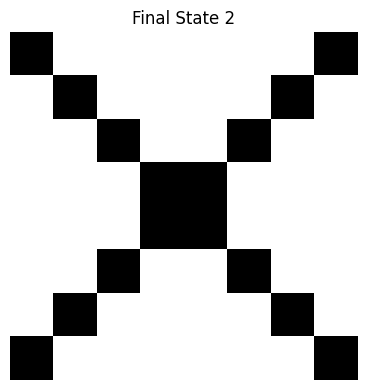
\includegraphics[width=\textwidth]{Final State 2.png}
\caption{Final State 2}
\end{subfigure}

\begin{subfigure}{0.2\textwidth}
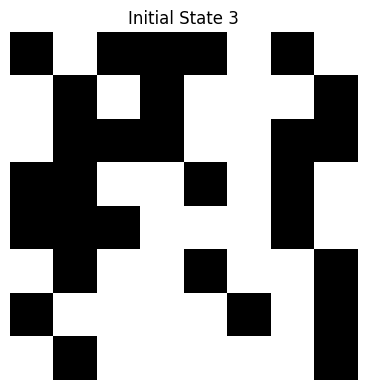
\includegraphics[width=\textwidth]{Initial State 3.png}
\caption{Initial State 3}
\end{subfigure}
\begin{subfigure}{0.2\textwidth}
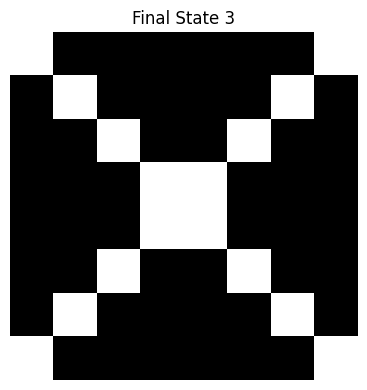
\includegraphics[width=\textwidth]{Final State 3.png}
\caption{Final State 3}
\end{subfigure}
\caption{Three simulations with different random initial states. All converge to fixed points close to the stored 'X' pattern.}
\label{fig:fixed_points}
\end{figure}

Multiple simulations with different initial conditions revealed the fixed points of the system. As predicted by theory, with one stored pattern $p$, the network exhibits two fixed points: the pattern itself and its negative (-$p$).

The stability of these fixed points was evident from the convergence behavior of the network. All initial states converged to one of these fixed points, depending on which basin of attraction they started in. This behavior is characteristic of associative memory systems.

% The overlap between each final state and the stored pattern was calculated using:
% \begin{equation}
% \text{overlap} = \frac{1}{N}\sum_{i=1}^{N}x_i p_i
% \end{equation}

% Across multiple trials, the final states consistently show high overlap with the stored pattern (approximately 0.9-1.0), confirming that the stored pattern acts as an attractor in the network's state space.

\subsection{Introduce a new pattern}

To test multiple pattern storage, I created and added a second pattern—a smiley face (\smiley{})—to the network:

\begin{figure}[H]
\centering

\includegraphics[width=0.3\textwidth]{Pattern 'Smiley'.png}
\caption{Visual representation of the second pattern (\smiley{}) stored in the network.}
\label{fig:pattern2}
\end{figure}

After adding the second pattern, the weight matrix was updated according to:
\begin{equation}
W = \frac{1}{N}(pp^T + qq^T)
\end{equation}
where $p$ is the 'X' pattern and $q$ is the \smiley{} pattern.

\begin{figure}[H]
\centering
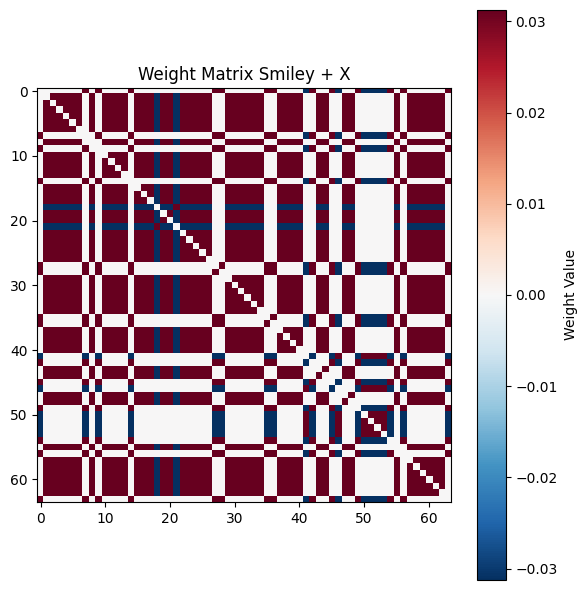
\includegraphics[width=0.3\textwidth]{Weight Matrix Smiley + X.png}
\caption{Updated weight matrix after storing both 'X' and \smiley{} patterns.}
\label{fig:weight_matrix2}
\end{figure}

The updated weight matrix now encodes information about both patterns, with more complex connection patterns reflecting the correlations between neurons in both stored patterns.


\subsubsection{Dynamics with Multiple Patterns}
With two stored patterns, the network exhibits four potential fixed points: the two patterns and their negatives. The convergence behavior became more complex, as initial states could now be attracted to any of these fixed points based on their proximity in the state space.
% When simulating the network with random initial conditions after storing two patterns, we observe that the network tends to converge to one of the stored patterns:

\begin{figure}[H]
\centering
\begin{subfigure}[b]{0.95\textwidth}
    \centering
    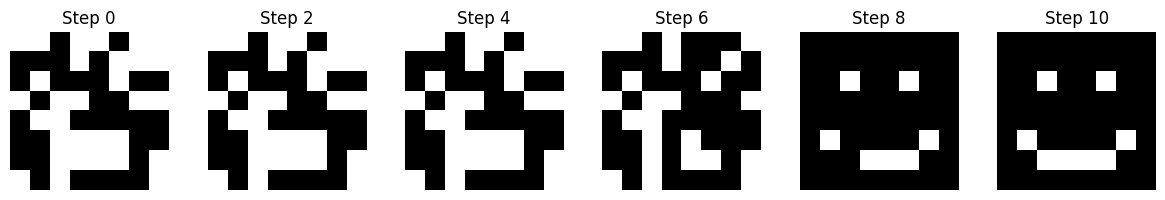
\includegraphics[width=0.95\textwidth]{Network Converge Smiley.png}
    \caption{Evolution of network activity from random initial conditions converging to the smiley pattern.}
    \label{fig:converge_smiley}
\end{subfigure}

\vspace{0.5cm}
\begin{subfigure}[b]{0.95\textwidth}
    \centering
    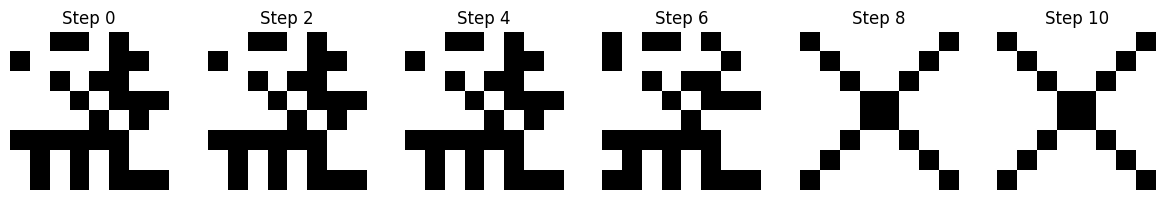
\includegraphics[width=0.95\textwidth]{Network Converge X.png}
    \caption{Evolution of network activity from different random initial conditions converging to the X pattern.}
    \label{fig:converge_x}
\end{subfigure}

\caption{Network dynamics with two stored patterns. Different initial conditions lead to convergence to different stored patterns, demonstrating multiple attractor basins in the network.}
\label{fig:dual_convergence}
\end{figure}

% The overlap calculations with both patterns reveal which attractor captured the network dynamics:
% \begin{align}
% \text{Overlap with 'X' pattern} &= 0.xxxx \\
% \text{Overlap with \smiley{} pattern} &= 0.yyyy
% \end{align}

These results demonstrate that with multiple patterns stored, the network state space contains multiple attractors, and the dynamics converge to the attractor basin of the pattern most similar to the initial conditions.


\subsection{Initial conditions}

One of the key properties of Hopfield networks is their ability to recover patterns from corrupted or noisy inputs. I tested this by creating a corrupted version of the 'X' pattern with 30\% of its bits flipped:

% \begin{figure}[H]
% \centering
% 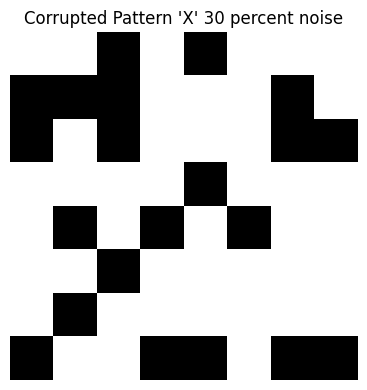
\includegraphics[width=0.4\textwidth]{Corrupted Pattern 'X' 30 percent noise.png}
% \caption{The 'X' pattern corrupted with 30\% noise.}
% \label{fig:corrupted}
% \end{figure}

Using this corrupted pattern as the initial state, I simulated the network dynamics:

\begin{figure}[H]
\centering
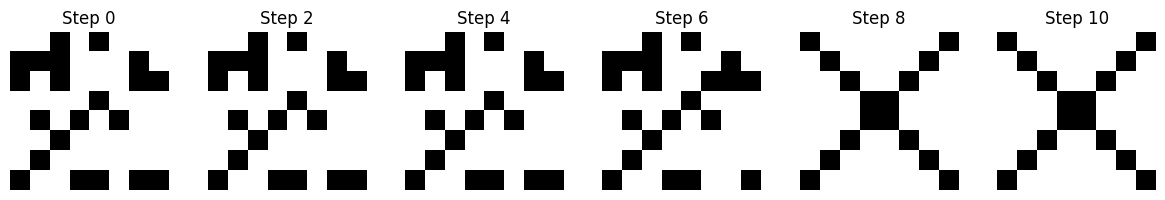
\includegraphics[width=0.9\textwidth]{Network Activity Corrupted X.png}
\caption{Network dynamics starting from the corrupted pattern. The network successfully recovers the original pattern.}
\label{fig:recovery}
\end{figure}

The network successfully recovered the original pattern, demonstrating the error-correction capabilities of the Hopfield network.


\subsection{Network capacity}

The theoretical storage capacity of a Hopfield network is approximately $0.138N$ patterns, where $N$ is the number of neurons. For our network with $N=64$, this gives a theoretical capacity of about 9 patterns.

To empirically test the network's capacity, I conducted multiple trials with an increasing number of random patterns stored in the network. For each pattern count, I measured the recovery success rate by corrupting each pattern and checking if the network could successfully recover it:

\begin{figure}[H]
\centering
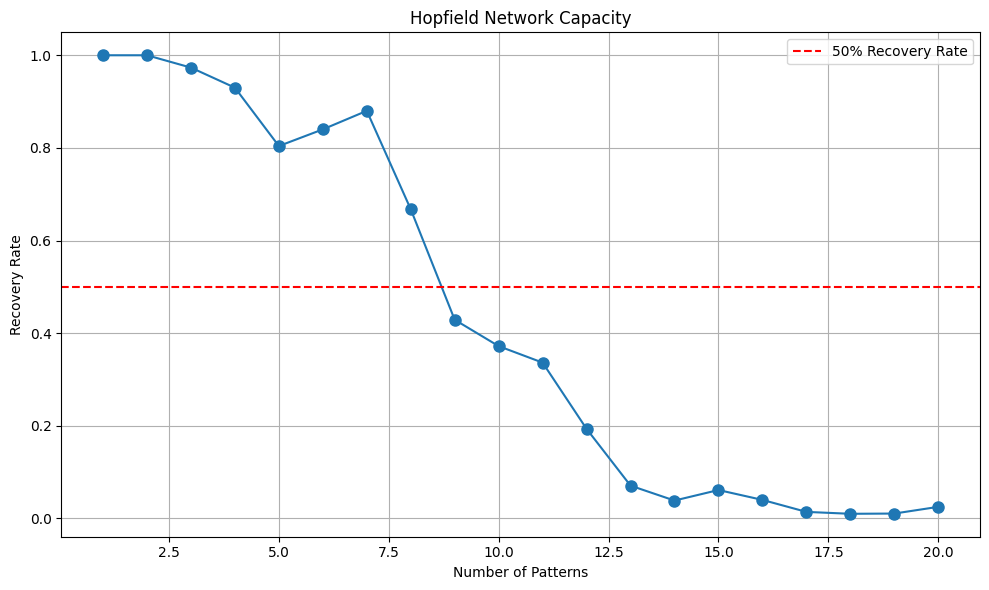
\includegraphics[width=0.8\textwidth]{capacity_curve.png}
\caption{Network capacity curve showing recovery rate vs. number of stored patterns.}
\label{fig:capacity}
\end{figure}

The results show that the recovery rate remains high (above 95\%) when storing up to approximately 7-8 patterns. Beyond that, the recovery rate drops rapidly, crossing the 50\% threshold at around 9 patterns, which aligns well with the theoretical capacity of $0.138 \times 64 \approx 9$ patterns.

This decline in performance occurs because as more patterns are stored, they begin to interfere with each other in the weight matrix, creating spurious attractors and reducing the basin of attraction for each stored pattern.



\section{Conclusion}

% \paragraph{Synthesis of Results}
This homework shows that scaling up one simple idea—\emph{positive feedback paired with an S-shaped activation function}—turns small circuits into stronger memory devices.  
\begin{itemize}
    \item A single self-exciting neuron (Figs.\,1–5) already behaves like a two-state switch.  
    \item A pair of mutually exciting neurons (Figs.\,6–9) embeds the same switch in a two-dimensional state space.  
    \item A 64-unit Hopfield network (Figs.\,10–19) pushes the principle further, forming an associative memory that stores and retrieves full patterns.  
\end{itemize}
In every case, the key is the appearance of \emph{multiple attractors}, which give the circuit a stable way to hold information over time.

\subsubsection*{1.\;Self-Connected Neuron (Figures 1–5)}
A single neuron with a sigmoidal transfer curve (Figure 1) becomes a compact memory switch when it feeds back onto itself: the feedback creates three fixed points—two stable equilibria (quiescent and high-rate) separated by an unstable threshold (flux plot, Figure 4). Random fluctuations occasionally push the firing rate across this threshold, and the jump frequency rises with noise amplitude (Figure 3). Together, these results show that an self-connected neuron alone can implement a robust yet tunable two-state memory element.


\subsubsection*{2.\;Two Neurons with Mutual Excitation (Figures 6–9)}
In a reciprocally exciting two-neuron module, state space analysis reveals three fixed points—a low-rate node, a saddle, and a high-rate node—whose stability classes are confirmed by the eigenvalues of the Jacobian matrix (Figure 8). The saddle’s one-dimensional stable manifold acts as a separatrix, partitioning state space so that trajectories flow either toward global quiescence or toward a self-sustained high-activity state, as illustrated by the vector field in Figure 7. When the external input current is strongly negative, the low-rate node is the sole attractor; however, as the tonic drive~$I$ is increased past a critical value ($I \approx -16$), a saddle–node bifurcation creates a saddle–high-rate pair, switching the circuit from monostable to bistable dynamics (Figure 9). Thus, the microcircuit functions as a neural flip-flop whose mode—monostable or bistable—can be tuned by the level of external drive.


\subsubsection*{3.\;Hopfield Network (Figures 10–19)}

Storing a single prototype in a Hopfield network produces two global
attractors—the pattern itself and its complement—so random initial
states reliably converge to whichever basin is closer (Figure~13).
Adding a second prototype doubles the attractor count to four
(Figure~16) and still allows the network to reconstruct images
containing up to 30\,\% corrupted pixels (Figures~17).  Systematic
capacity tests (Figure~18) confirm the classic limit of roughly
$0.138N$ stable memories (about nine for the present $N=64$ network);
beyond this point, interference creates spurious minima and sharply
reduces recall accuracy. these findings show that the
Hopfield architecture scales the bistable switch into a high-dimensional
associative memory whose performance is both powerful and predictably
bounded.

% \subsection*{Broader Significance}
% Across cellular, microcircuit, and network scales, \emph{recurrent excitation coupled with a nonlinear response curve} consistently yields multiple, stable activity states.  Such attractor dynamics provide a unifying computational substrate for working memory, decision thresholds, and error-correcting pattern completion in both biological and artificial neural systems.  Analytical tools—state space geometry, bifurcation tracking, and Lyapunov-style energy functions—afford precise control over these dynamics and thereby inform the principled design of memory circuits with desired stability–flexibility trade-offs.

\end{document}
